% !TEX TS-program = pdflatex
% !TEX encoding = UTF-8 Unicode

\documentclass[preprint]{sigplanconf}

\usepackage{graphicx,listings,fixltx2e}

\begin{document}
\conferenceinfo{PLDI 2011}{June 4--8, 2011, San Jose, CA, USA.}
\copyrightyear{2010}

\preprintfooter{PLDI 2011}
\titlebanner{DRAFT---Do not distribute}

\title{Parakeet: General Purpose GPU Programming with High Level Array
Languages}
\authorinfo{Anonymous}{Anonymous}{Anonymous}

\maketitle

\begin{abstract}
Contemporary GPUs offer staggering performance potential, which has
led to an explosion in recent work on enabling the execution of
general-purpose programs on GPUs. Despite various advances in making
general-purpose GPU programming easier, the two commonly used
frameworks (NVIDIA's CUDA and OpenCL) are cumbersome and require
detailed architectural knowledge on the part of the programmer to
fully harness this performance potential.

The potential performance advantage over contemporary CPUs that GPUs
offer is due in large part to their having been heavily optimized for
data parallel workloads.  Array-oriented programming--which encourages
the use of data parallel array operators (e.g.\ map, reduce, and
scan), and de-emphasizes the importance of explicit loops--is thus a
natural model for high level programming of GPUs.

We present Parakeet, an intelligent runtime for executing high level
array-oriented programs on GPUs.  The heart of Parakeet is an
interpreter, which upon reaching an array operator synthesizes and
executes a GPU program to implement that operator. Parakeet takes
advantage of runtime information both to choose between different
possible implementations of a GPU program and to set execution
parameters which greatly impact performance. Parakeet transparently
moves data to and from the GPU and performs garbage collection of GPU
memory.

We evaluate our system on two standard benchmarks: Black-Scholes
option pricing, and K-Means clustering.  We compare high level
array-oriented implementations to hand-written tuned GPU versions from
the CUDA SDK and the Rodinia GPU benchmark suite. Despite having
orders of magnitude less code, the high level
versions perform competitively when executed by Parakeet.
\end{abstract}

\section{Introduction}

Contemporary GPUs boast massive performance potential--in some cases orders of
magnitude higher performance per dollar than that of CPUs--and most desktop
systems today come with graphics processors.  This has led to an explosion in
recent work on enabling the execution of general-purpose programs on GPUs
(GPGPU) in order to harness this performance for non-graphics tasks
\cite{Cata10,Main10,Muns10,NvidCU,Sven08,Tard06}. Despite this, the two widely
used GPGPU frameworks--NVIDIA's CUDA \cite{NvidCU} and OpenCL
\cite{Muns10}--require the programmer to use extensive knowledge of low level
architectural details in order to fully harness the performance potential.
While this might be acceptable for well-trained systems hackers, professionals
in other domains such as the natural sciences who could potentially
benefit from the performance boost from using GPUs are unable to do so.

% Enable programmers to write GPGPU programs in productivity language
Our goal is to lower the barrier on GPGPU programming by
enabling programmers to use productivity languages for writing
efficient GPGPU programs. Productivity languages, such as Python or Matlab,
trade off program speed in order to allow programmers to write code more quickly
and with less effort than efficiency languages such as C.  We aim to deliver
both performance and ease of use by focusing on a specific class of parallel
computation: data parallelism.  Data parallelism is present in many important
algorithms and problem domains, e.g.\ machine learning and linear algebra, and
has been well studied in the literature (e.g.\ in \cite{Blel90}).  Data
parallelism is also a natural
model for GPU programming, as much of the performance advantage GPUs offer over
CPUs comes from their having been heavily optimized for data parallel workloads.
 We thus target languages with support for \emph{array-oriented programming}.
Array-oriented programming encourages the use of data parallel array operators
(such as map, reduce, and scan) for operating on first-class array types, and
de-emphasizes the importance of explicit loops.

% Heart of Parakeet - an interpreter for our high level IL w/ array ops
In this paper, we present Parakeet, an intelligent runtime for executing high
level array-oriented programs on GPUs.  The core of Parakeet is an interpreter
for its high level, typed intermediate language that includes native support for
array operators.  When the Parakeet interpreter reaches an array operator such
as {\tt Map}, it uses dynamic runtime information to decide whether to
synthesize a GPU program to implement that operator, taking advantage of the
GPU transparently to the programmer.

% Agnosticism
Parakeet is agnostic as to the source language used by the programmer, provided
that the language has support for the required array operators.  We have
implemented the first front end for the Parakeet system for Q, a high level,
dynamically typed array language derived from APL and widely used in financial
computing \cite{Borr08}. Parakeet's first back end is for PTX, the
pseudoassembly language used by NVIDIA GPUs \cite{NvidCU}.  We are currently
working on front ends for data parallel subsets of Matlab and Python, and plan
on supporting multicore CPUs in the future as well.

% Pipeline of execution
The pipeline of the execution of a program begins by the Parakeet system
intercepting function calls from the source language's interpreter and type
specializing them according to their argument types.  Parakeet then performs
various standard compiler optimizations on this IL form of the functions, as
well as fusion of array operators which is very beneficial for performance.
Parakeet then interprets the typed function, selectively executing array
operators either on the GPU or CPU. Parakeet synthesizes GPU
programs from a library of efficient array operator implementation skeletons,
with splice points where user-defined functions get inlined. Parakeet supports
the nesting of array operators, using heuristics to decide which level of
nesting should be compiled to GPU kernels, with the outer levels of nesting are
translated into iterative kernel invocations by our CPU runtime.  Data movement
and GPU garbage collection are handled transparently by Parakeet.

% Performance
We evaluate Parakeet on two standard benchmark programs: Black-Scholes option
pricing and K-Means clustering.  We compare Q implementations of these
benchmarks run by Parakeet to hand-written, tuned GPU and CPU implementations
from the Rodinia \cite{Che09} and Parsec \cite{Bien08} benchmark suites and the
NVIDIA CUDA SDK \cite{NvidSD}.  Despite the Q implementations requiring orders
of magnitude fewer lines of code, our system delivers competitive performance.

% Bullet-point, drive-home contributions
The main contributions of this paper are the following:

\begin{itemize}
\item A working system in which programmers can write complex, high level code
that is automatically parallelized into efficient GPU programs.
\item A series of high-level fusion optimization rules for higher-order data
parallel operators.
\item Evidence that dynamic compilation of GPU programs can significantly
improve their performance by taking advantage of runtime information to
tailor their code and execution to runtime information.
\end{itemize}

\section{Parakeet's Intermediate Language}

There's going to be a lot of text and code examples in this section.  I want to
push the Q examples down further, so that we see the bullet points from the
Intro section where they belong.  Hence the following ipso.

There's going to be a lot of text and code examples in this section.  I want to
push the Q examples down further, so that we see the bullet points from the
Intro section where they belong.  Hence the following ipso.There's going to be a
lot of text and code examples in this section.  I want to
push the Q examples down further, so that we see the bullet points from the
Intro section where they belong.  Hence the following ipso.There's going to be a
lot of text and code examples in this section.  I want to
push the Q examples down further, so that we see the bullet points from the
Intro section where they belong.  Hence the following ipso.There's going to be a
lot of text and code examples in this section.  I want to
push the Q examples down further, so that we see the bullet points from the
Intro section where they belong.  Hence the following ipso.There's going to be a
lot of text and code examples in this section.  I want to
push the Q examples down further, so that we see the bullet points from the
Intro section where they belong.  Hence the following ipso.There's going to be a
lot of text and code examples in this section.  I want to
push the Q examples down further, so that we see the bullet points from the
Intro section where they belong.  Hence the following ipso.There's going to be a
lot of text and code examples in this section.  I want to
push the Q examples down further, so that we see the bullet points from the

Intro section where they belong.  Hence the following ipso.There's going to be a
lot of text and code examples in this section.  I want to
push the Q examples down further, so that we see the bullet points from the
Intro section where they belong.  Hence the following ipso.There's going to be a
lot of text and code examples in this section.  I want to
push the Q examples down further, so that we see the bullet points from the
Intro section where they belong.  Hence the following ipso.There's going to be a
lot of text and code examples in this section.  I want to
push the Q examples down further, so that we see the bullet points from the
Intro section where they belong.  Hence the following ipso.There's going to be a
lot of text and code examples in this section.  I want to
push the Q examples down further, so that we see the bullet points from the
Intro section where they belong.  Hence the following ipso.There's going to be a
lot of text and code examples in this section.  I want to
push the Q examples down further, so that we see the bullet points from the
Intro section where they belong.  Hence the following ipso.There's going to be a
lot of text and code examples in this section.  I want to
push the Q examples down further, so that we see the bullet points from the
Intro section where they belong.  Hence the following ipso.There's going to be a
lot of text and code examples in this section.  I want to
push the Q examples down further, so that we see the bullet points from the
Intro section where they belong.  Hence the following ipso.There's going to be a
lot of text and code examples in this section.  I want to
push the Q examples down further, so that we see the bullet points from the
Intro section where they belong.  Hence the following ipso.There's going to be a
lot of text and code examples in this section.  I want to
push the Q examples down further, so that we see the bullet points from the
Intro section where they belong.  Hence the following ipso.There's going to be a
lot of text and code examples in this section.  I want to
push the Q examples down further, so that we see the bullet points from the
Intro section where they belong.  Hence the following ipso.There's going to be a
lot of text and code examples in this section.  I want to
push the Q examples down further, so that we see the bullet points from the
Intro section where they belong.  Hence the following ipso.There's going to be a
lot of text and code examples in this section.  I want to
push the Q examples down further, so that we see the bullet points from the
Intro section where they belong.  Hence the following ipso.There's going to be a
lot of text and code examples in this section.  I want to
push the Q examples down further, so that we see the bullet points from the
Intro section where they belong.  Hence the following ipso.There's going to be a
lot of text and code examples in this section.  I want to


push the Q examples down further, so that we see the bullet points from the
Intro section where they belong.  Hence the following ipso.There's going to be a
lot of text and code examples in this section.  I want to
push the Q examples down further, so that we see the bullet points from the
Intro section where they belong.  Hence the following ipso.There's going to be a
lot of text and code examples in this section.  I want to
push the Q examples down further, so that we see the bullet points from the
Intro section where they belong.  Hence the following ipso.There's going to be a
lot of text and code examples in this section.  I want to
push the Q examples down further, so that we see the bullet points from the
Intro section where they belong.  Hence the following ipso.There's going to be a
lot of text and code examples in this section.  I want to
push the Q examples down further, so that we see the bullet points from the
Intro section where they belong.  Hence the following ipso.There's going to be a
lot of text and code examples in this section.  I want to
push the Q examples down further, so that we see the bullet points from the
Intro section where they belong.  Hence the following ipso.There's going to be a
lot of text and code examples in this section.  I want to
push the Q examples down further, so that we see the bullet points from the
Intro section where they belong.  Hence the following ipso.There's going to be a
lot of text and code examples in this section.  I want to

push the Q examples down further, so that we see the bullet points from the
Intro section where they belong.  Hence the following ipso.There's going to be a
lot of text and code examples in this section.  I want to
push the Q examples down further, so that we see the bullet points from the
Intro section where they belong.  Hence the following ipso.There's going to be a
lot of text and code examples in this section.  I want to
push the Q examples down further, so that we see the bullet points from the
Intro section where they belong.  Hence the following ipso.There's going to be a
lot of text and code examples in this section.  I want to
push the Q examples down further, so that we see the bullet points from the
Intro section where they belong.  Hence the following ipso.There's going to be a
lot of text and code examples in this section.  I want to
push the Q examples down further, so that we see the bullet points from the
Intro section where they belong.  Hence the following ipso.There's going to be a
lot of text and code examples in this section.  I want to

push the Q examples down further, so that we see the bullet points from the
Intro section where they belong.  Hence the following ipso.There's going to be a
lot of text and code examples in this section.  I want to
push the Q examples down further, so that we see the bullet points from the
Intro section where they belong.  Hence the following ipso.There's going to be a
lot of text and code examples in this section.  I want to
push the Q examples down further, so that we see the bullet points from the
Intro section where they belong.  Hence the following ipso.There's going to be a
lot of text and code examples in this section.  I want to
push the Q examples down further, so that we see the bullet points from the
Intro section where they belong.  Hence the following ipso.There's going to be a
lot of text and code examples in this section.  I want to
push the Q examples down further, so that we see the bullet points from the
Intro section where they belong.  Hence the following ipso.There's going to be a
lot of text and code examples in this section.  I want to
push the Q examples down further, so that we see the bullet points from the
Intro section where they belong.  Hence the following ipso.There's going to be a
lot of text and code examples in this section.  I want to
push the Q examples down further, so that we see the bullet points from the
Intro section where they belong.  Hence the following ipso.There's going to be a
lot of text and code examples in this section.  I want to

push the Q examples down further, so that we see the bullet points from the
Intro section where they belong.  Hence the following ipso.There's going to be a
lot of text and code examples in this section.  I want to
push the Q examples down further, so that we see the bullet points from the
Intro section where they belong.  Hence the following ipso.There's going to be a
lot of text and code examples in this section.  I want to
push the Q examples down further, so that we see the bullet points from the
Intro section where they belong.  Hence the following ipso.There's going to be a
lot of text and code examples in this section.  I want to
push the Q examples down further, so that we see the bullet points from the
Intro section where they belong.  Hence the following ipso.There's going to be a
lot of text and code examples in this section.  I want to
push the Q examples down further, so that we see the bullet points from the
Intro section where they belong.  Hence the following ipso.There's going to be a
lot of text and code examples in this section.  I want to
push the Q examples down further, so that we see the bullet points from the
Intro section where they belong.  Hence the following ipso.There's going to be a
lot of text and code examples in this section.  I want to
push the Q examples down further, so that we see the bullet points from the
Intro section where they belong.  Hence the following ipso.There's going to be a
lot of text and code examples in this section.  I want to
push the Q examples down further, so that we see the bullet points from the
Intro section where they belong.  Hence the following ipso.There's going to be a
lot of text and code examples in this section.  I want to

push the Q examples down further, so that we see the bullet points from the
Intro section where they belong.  Hence the following ipso.There's going to be a
lot of text and code examples in this section.  I want to
push the Q examples down further, so that we see the bullet points from the
Intro section where they belong.  Hence the following ipso.There's going to be a
lot of text and code examples in this section.  I want to
push the Q examples down further, so that we see the bullet points from the
Intro section where they belong.  Hence the following ipso.There's going to be a
lot of text and code examples in this section.  I want to
push the Q examples down further, so that we see the bullet points from the
Intro section where they belong.  Hence the following ipso.There's going to be a
lot of text and code examples in this section.  I want to
push the Q examples down further, so that we see the bullet points from the
Intro section where they belong.  Hence the following ipso.There's going to be a
lot of text and code examples in this section.  I want to
push the Q examples down further, so that we see the bullet points from the
Intro section where they belong.  Hence the following ipso.There's going to be a
lot of text and code examples in this section.  I want to
push the Q examples down further, so that we see the bullet points from the
Intro section where they belong.  Hence the following ipso.There's going to be a
lot of text and code examples in this section.  I want to
push the Q examples down further, so that we see the bullet points from the
Intro section where they belong.  Hence the following ipso.There's going to be a
lot of text and code examples in this section.  I want to
push the Q examples down further, so that we see the bullet points from the
Intro section where they belong.  Hence the following ipso.There's going to be a
lot of text and code examples in this section.  I want to
push the Q examples down further, so that we see the bullet points from the
Intro section where they belong.  Hence the following ipso.

\section{Q: A High-Level Array Language}
\label{Q}

While we emphasize that the Parakeet framework is largely source language
agnostic, we chose to implement its first front end for Q, a high-level,
sequential array programming language from the APL family \cite{Borr08}.
Q is dynamically typed, and the standard proprietary implementation is
interpreted. Q is a natural choice for Parakeet, since idiomatic Q code uses
native array types and a rich set of array operators and higher-order
data parallel function modifiers that map well onto the Parakeet array
operators. Q is also a fully-featured language, with a large library of built-in
functions, and has a large user base in financial computing. Since our
focus is the Parakeet runtime, we omit many details of the Q language and only
present the salient features so as to illustrate the level of programming
and Q's support for array operators, as well as to make our later code examples
clear.

\subsection{Q Examples}
\begin{figure}
\begin{verbatim}
1  f: {[x] 5 + 3 * x}
2
3  / Create input array
4  a: til 10000
5
6  / Call f on different inputs
7  b: f[6]
8  c: f[a]
\end{verbatim}
\caption{Q Map Example}
\label{QMap}
\end{figure}

Figure \ref{QMap} gives an example of a simple Q program.  In line 1, we define
a function \texttt{f} which takes a single argument \texttt{x} and computes a
simple linear function of it.  In Q syntax, the colon operator is used for
assignment, and curly braces surround function definitions.  Brackets are used
to declare function arguments, with semicolons serving as list delimiters
between the various arguments.  Q functions return the result of their final
statement.  On line 3 we see a comment, denoted by a single \texttt{/}, and on
line 4 we use the built-in function \texttt{til} to generate a
100000-element array of integers ranging from \texttt{0} to \texttt{999999}.

In line 7, we finally perform our first computation, evaluating \texttt{f} on
the input \texttt{6} with the bracket function call syntax, storing the
value \texttt{23} in variable \texttt{b}.  Line 8 evaluates \texttt{f}
element-wise on the entire array \texttt{a}, storing the result in \texttt{c}.

This code snippet illustrates a key feature of Q for our purposes.  Functions
are agnostic to the shape of their input arguments--as we saw, \texttt{f} was
legally applied both to a scalar input as well as to an array.  In effect, the
function \texttt{f} was {\it mapped} element-wise over the array \texttt{a}.
Thus we see that Q programs can express data parallel computations in a compact,
declarative, high level fashion.  No explicit looping over the elements of
\texttt{a} is required.

\begin{figure}
\begin{verbatim}
1  a: til 10000
2
3  b: 0 +/ a
4  c: 0 +\ a
\end{verbatim}
\caption{Q Reductions Example}
\label{QReduce}
\end{figure}

In Figure \ref{QReduce}, we introduce the concept of an \emph{adverb}.  Q has a
series of adverbs, which are higher-order function modifiers.  In
line 3, we see an example of the reduction adverb, denoted with the syntax
`\texttt{/}', which modifies a binary function. When the modified function is
then applied to an array input, the result is as though the function was
inserted infix between all elements of the array.  Thus this adverb corresponds
to the \texttt{Reduce} array operator of the Parakeet language.  The reduce
adverb also takes an initial value argument, which is treated as though it were
prepended to the input of the reduce.  Thus, after executing line 3 \texttt{b}
will contain the sum of the array \texttt{a}.

In line 4, we see the \emph{scan} adverb, with syntax `\texttt{\char`\\}'.
Scan computes the running value of the function it modifies when applied
element-per-element to an input array. Scan also takes an initial value
argument.  In Parakeet, this corresponds to the \texttt{Scan} array operator,
which as emphasized in \cite{Blel90}, is very useful as a building block in many
parallel algorithms.

\begin{figure}
\begin{verbatim}
1  sqr: {[x] x*x}
2  dist: {[x;y] sqrt sum sqr x - y}
3
4  / Generate two 100x100 matrices
5  a: (100;100) # til 10000
6  b: (100;100) # til 10000
7
8  all_dists: dist/:\:[a;b]
\end{verbatim}
\caption{Q All-Pairs Distance Example}
\label{QAllPairsDist}
\end{figure}

In Figure \ref{QAllPairsDist}, we see a slightly more complicated example.
First we define a pair of functions--one that computes the square of an input
variable, and another that computes the Euclidean distance of two input
vectors.  The \texttt{sum} function used in the \texttt{dist} function body is a
built-in reduction function, which computes the sum of all elements of its input
argument.  The \texttt{dist} function also illustrates that Q code is evaluated
\emph{left of right}--the input vectors \texttt{x} and \texttt{y} are
subtracted, then their square is computed, this is summed, and finally the
square root of this sum is returned.

In lines 5 and 6, we generate two 100x100 matrices.  The \texttt{\#} operator is
used to modify the shape of a variable: its left argument is a list of lengths
for the dimensions, and the right argument is a variable whose shape is to be
modified.  Lists in Q are enclosed in parentheses.

In line 8, we evaluate the \texttt{dist} function on the matrices \texttt{a} and
\texttt{b} using the {\it all pairs} adverb (corresponding to the
\texttt{AllPairs} Parakeet array operator).  This adverb--which is technically
a combination of the adverbs \emph{left-each} (\texttt{/:}) and
\emph{right-each} (\texttt{\char`\\:})--applies its function argument to all
pairs of each of its inputs--in this case, all pairs of rows from \texttt{a} and
rows from \texttt{b}.  The resulting \texttt{all\_dists} variable will contain a
matrix of all the Euclidean distances between rows of \texttt{a} and \texttt{b}.

\section{Compilation Pipeline}
\label{Compilation}

Do All-Pairs distances here.

Here's some placeholder text for the compilation pipeline section.  This
section should easily take up the most of any section, around 2.5-3 pages I
would imagine.
Here's some placeholder text for the compilation pipeline section.  This
section should easily take up the most of any section, around 2.5-3 pages I
would imagine.Here's some placeholder text for the compilation pipeline section.
 This
section should easily take up the most of any section, around 2.5-3 pages I
would imagine.

Here's some placeholder text for the compilation pipeline section.  This
section should easily take up the most of any section, around 2.5-3 pages I
would imagine.
Here's some placeholder text for the compilation pipeline section.  This
section should easily take up the most of any section, around 2.5-3 pages I
would imagine.Here's some placeholder text for the compilation pipeline section.
 This
section should easily take up the most of any section, around 2.5-3 pages I
would imagine.
Here's some placeholder text for the compilation pipeline section.  This
section should easily take up the most of any section, around 2.5-3 pages I
would imagine.
Here's some placeholder text for the compilation pipeline section.  This
section should easily take up the most of any section, around 2.5-3 pages I
would imagine.Here's some placeholder text for the compilation pipeline section.
 This
section should easily take up the most of any section, around 2.5-3 pages I
would imagine.

Here's some placeholder text for the compilation pipeline section.  This
section should easily take up the most of any section, around 2.5-3 pages I
would imagine.
Here's some placeholder text for the compilation pipeline section.  This
section should easily take up the most of any section, around 2.5-3 pages I
would imagine.Here's some placeholder text for the compilation pipeline section.
 This
section should easily take up the most of any section, around 2.5-3 pages I
would imagine.
Here's some placeholder text for the compilation pipeline section.  This
section should easily take up the most of any section, around 2.5-3 pages I
would imagine.
Here's some placeholder text for the compilation pipeline section.  This
section should easily take up the most of any section, around 2.5-3 pages I
would imagine.Here's some placeholder text for the compilation pipeline section.
 This
section should easily take up the most of any section, around 2.5-3 pages I
would imagine.

Here's some placeholder text for the compilation pipeline section.  This
section should easily take up the most of any section, around 2.5-3 pages I
would imagine.
Here's some placeholder text for the compilation pipeline section.  This
section should easily take up the most of any section, around 2.5-3 pages I
would imagine.Here's some placeholder text for the compilation pipeline section.
 This
section should easily take up the most of any section, around 2.5-3 pages I
would imagine.
Here's some placeholder text for the compilation pipeline section.  This
section should easily take up the most of any section, around 2.5-3 pages I
would imagine.
Here's some placeholder text for the compilation pipeline section.  This
section should easily take up the most of any section, around 2.5-3 pages I
would imagine.Here's some placeholder text for the compilation pipeline section.
 This
section should easily take up the most of any section, around 2.5-3 pages I
would imagine.
Here's some placeholder text for the compilation pipeline section.  This
section should easily take up the most of any section, around 2.5-3 pages I
would imagine.
Here's some placeholder text for the compilation pipeline section.  This
section should easily take up the most of any section, around 2.5-3 pages I
would imagine.Here's some placeholder text for the compilation pipeline section.
 This
section should easily take up the most of any section, around 2.5-3 pages I
would imagine.
Here's some placeholder text for the compilation pipeline section.  This
section should easily take up the most of any section, around 2.5-3 pages I
would imagine.
Here's some placeholder text for the compilation pipeline section.  This
section should easily take up the most of any section, around 2.5-3 pages I
would imagine.Here's some placeholder text for the compilation pipeline section.
 This
section should easily take up the most of any section, around 2.5-3 pages I
would imagine.

Here's some placeholder text for the compilation pipeline section.  This
section should easily take up the most of any section, around 2.5-3 pages I
would imagine.
Here's some placeholder text for the compilation pipeline section.  This
section should easily take up the most of any section, around 2.5-3 pages I
would imagine.Here's some placeholder text for the compilation pipeline section.
 This
section should easily take up the most of any section, around 2.5-3 pages I
would imagine.
Here's some placeholder text for the compilation pipeline section.  This
section should easily take up the most of any section, around 2.5-3 pages I
would imagine.
Here's some placeholder text for the compilation pipeline section.  This
section should easily take up the most of any section, around 2.5-3 pages I
would imagine.Here's some placeholder text for the compilation pipeline section.
 This
section should easily take up the most of any section, around 2.5-3 pages I
would imagine.

Here's some placeholder text for the compilation pipeline section.  This
section should easily take up the most of any section, around 2.5-3 pages I
would imagine.
Here's some placeholder text for the compilation pipeline section.  This
section should easily take up the most of any section, around 2.5-3 pages I
would imagine.Here's some placeholder text for the compilation pipeline section.
 This
section should easily take up the most of any section, around 2.5-3 pages I
would imagine.
Here's some placeholder text for the compilation pipeline section.  This
section should easily take up the most of any section, around 2.5-3 pages I
would imagine.
Here's some placeholder text for the compilation pipeline section.  This
section should easily take up the most of any section, around 2.5-3 pages I
would imagine.Here's some placeholder text for the compilation pipeline section.
 This
section should easily take up the most of any section, around 2.5-3 pages I
would imagine.

Here's some placeholder text for the compilation pipeline section.  This
section should easily take up the most of any section, around 2.5-3 pages I
would imagine.
Here's some placeholder text for the compilation pipeline section.  This
section should easily take up the most of any section, around 2.5-3 pages I
would imagine.Here's some placeholder text for the compilation pipeline section.
 This
section should easily take up the most of any section, around 2.5-3 pages I
would imagineHere's some placeholder text for the compilation pipeline section.
This
section should easily take up the most of any section, around 2.5-3 pages I
would imagine.
Here's some placeholder text for the compilation pipeline section.  This
section should easily take up the most of any section, around 2.5-3 pages I
would imagine.Here's some placeholder text for the compilation pipeline section.
 This
section should easily take up the most of any section, around 2.5-3 pages I
would imagine.
Here's some placeholder text for the compilation pipeline section.  This
section should easily take up the most of any section, around 2.5-3 pages I
would imagine.
Here's some placeholder text for the compilation pipeline section.  This
section should easily take up the most of any section, around 2.5-3 pages I
would imagine.Here's some placeholder text for the compilation pipeline section.
 This
section should easily take up the most of any section, around 2.5-3 pages I
would imagine.

Here's some placeholder text for the compilation pipeline section.  This
section should easily take up the most of any section, around 2.5-3 pages I
would imagine.
Here's some placeholder text for the compilation pipeline section.  This
section should easily take up the most of any section, around 2.5-3 pages I
would imagine.Here's some placeholder text for the compilation pipeline section.
 This
section should easily take up the most of any section, around 2.5-3 pages I
would imagine.
Here's some placeholder text for the compilation pipeline section.  This
section should easily take up the most of any section, around 2.5-3 pages I
would imagine.
Here's some placeholder text for the compilation pipeline section.  This
section should easily take up the most of any section, around 2.5-3 pages I
would imagine.Here's some placeholder text for the compilation pipeline section.
 This
section should easily take up the most of any section, around 2.5-3 pages I
would imagine.
Here's some placeholder text for the compilation pipeline section.  This
section should easily take up the most of any section, around 2.5-3 pages I
would imagine.
Here's some placeholder text for the compilation pipeline section.  This
section should easily take up the most of any section, around 2.5-3 pages I
would imagine.Here's some placeholder text for the compilation pipeline section.
 This
section should easily take up the most of any section, around 2.5-3 pages I
would imagine.
Here's some placeholder text for the compilation pipeline section.  This
section should easily take up the most of any section, around 2.5-3 pages I
would imagine.
Here's some placeholder text for the compilation pipeline section.  This
section should easily take up the most of any section, around 2.5-3 pages I
would imagine.Here's some placeholder text for the compilation pipeline section.
 This
section should easily take up the most of any section, around 2.5-3 pages I
would imagine.

Here's some placeholder text for the compilation pipeline section.  This
section should easily take up the most of any section, around 2.5-3 pages I
would imagine.
Here's some placeholder text for the compilation pipeline section.  This
section should easily take up the most of any section, around 2.5-3 pages I
would imagine.Here's some placeholder text for the compilation pipeline section.
 This
section should easily take up the most of any section, around 2.5-3 pages I
would imagine
Here's some placeholder text for the compilation pipeline section.  This
section should easily take up the most of any section, around 2.5-3 pages I
would imagine.
Here's some placeholder text for the compilation pipeline section.  This
section should easily take up the most of any section, around 2.5-3 pages I
would imagine.Here's some placeholder text for the compilation pipeline section.
 This
section should easily take up the most of any section, around 2.5-3 pages I
would imagine.
Here's some placeholder text for the compilation pipeline section.  This
section should easily take up the most of any section, around 2.5-3 pages I
would imagine.
Here's some placeholder text for the compilation pipeline section.  This
section should easily take up the most of any section, around 2.5-3 pages I
would imagine.Here's some placeholder text for the compilation pipeline section.
 This
section should easily take up the most of any section, around 2.5-3 pages I
would imagine.

Here's some placeholder text for the compilation pipeline section.  This
section should easily take up the most of any section, around 2.5-3 pages I
would imagine.
Here's some placeholder text for the compilation pipeline section.  This
section should easily take up the most of any section, around 2.5-3 pages I
would imagine.Here's some placeholder text for the compilation pipeline section.
 This
section should easily take up the most of any section, around 2.5-3 pages I
would imagine.
Here's some placeholder text for the compilation pipeline section.  This
section should easily take up the most of any section, around 2.5-3 pages I
would imagine.
Here's some placeholder text for the compilation pipeline section.  This
section should easily take up the most of any section, around 2.5-3 pages I
would imagine.Here's some placeholder text for the compilation pipeline section.
 This
section should easily take up the most of any section, around 2.5-3 pages I
would imagine.Here's some placeholder text for the compilation pipeline section.
 This
section should easily take up the most of any section, around 2.5-3 pages I
would imagine.
Here's some placeholder text for the compilation pipeline section.  This
section should easily take up the most of any section, around 2.5-3 pages I
would imagine.Here's some placeholder text for the compilation pipeline section.
 This
section should easily take up the most of any section, around 2.5-3 pages I
would imagine.
Here's some placeholder text for the compilation pipeline section.  This
section should easily take up the most of any section, around 2.5-3 pages I
would imagine.
Here's some placeholder text for the compilation pipeline section.  This
section should easily take up the most of any section, around 2.5-3 pages I
would imagine.Here's some placeholder text for the compilation pipeline section.
 This
section should easily take up the most of any section, around 2.5-3 pages I
would imagine.

Here's some placeholder text for the compilation pipeline section.  This
section should easily take up the most of any section, around 2.5-3 pages I
would imagine.
Here's some placeholder text for the compilation pipeline section.  This
section should easily take up the most of any section, around 2.5-3 pages I
would imagine.Here's some placeholder text for the compilation pipeline section.
 This
section should easily take up the most of any section, around 2.5-3 pages I
would imagine
Here's some placeholder text for the compilation pipeline section.  This
section should easily take up the most of any section, around 2.5-3 pages I
would imagine.
Here's some placeholder text for the compilation pipeline section.  This
section should easily take up the most of any section, around 2.5-3 pages I
would imagine.Here's some placeholder text for the compilation pipeline section.
 This
section should easily take up the most of any section, around 2.5-3 pages I
would imagine.
Here's some placeholder text for the compilation pipeline section.  This
section should easily take up the most of any section, around 2.5-3 pages I
would imagine.
Here's some placeholder text for the compilation pipeline section.  This
section should easily take up the most of any section, around 2.5-3 pages I
would imagine.Here's some placeholder text for the compilation pipeline section.
 This
section should easily take up the most of any section, around 2.5-3 pages I
would imagine.

Here's some placeholder text for the compilation pipeline section.  This
section should easily take up the most of any section, around 2.5-3 pages I
would imagine.
Here's some placeholder text for the compilation pipeline section.  This
section should easily take up the most of any section, around 2.5-3 pages I
would imagine.Here's some placeholder text for the compilation pipeline section.
 This
section should easily take up the most of any section, around 2.5-3 pages I
would imagine.
Here's some placeholder text for the compilation pipeline section.  This
section should easily take up the most of any section, around 2.5-3 pages I
would imagine.
Here's some placeholder text for the compilation pipeline section.  This
section should easily take up the most of any section, around 2.5-3 pages I
would imagine.Here's some placeholder text for the compilation pipeline section.
 This
section should easily take up the most of any section, around 2.5-3 pages I
would imagine.
Here's some placeholder text for the compilation pipeline section.  This
section should easily take up the most of any section, around 2.5-3 pages I
would imagine.
Here's some placeholder text for the compilation pipeline section.  This
section should easily take up the most of any section, around 2.5-3 pages I
would imagine.Here's some placeholder text for the compilation pipeline section.
 This
section should easily take up the most of any section, around 2.5-3 pages I
would imagine.
Here's some placeholder text for the compilation pipeline section.  This
section should easily take up the most of any section, around 2.5-3 pages I
would imagine.
Here's some placeholder text for the compilation pipeline section.  This
section should easily take up the most of any section, around 2.5-3 pages I
would imagine.Here's some placeholder text for the compilation pipeline section.
 This
section should easily take up the most of any section, around 2.5-3 pages I
would imagine.

Here's some placeholder text for the compilation pipeline section.  This
section should easily take up the most of any section, around 2.5-3 pages I
would imagine.
Here's some placeholder text for the compilation pipeline section.  This
section should easily take up the most of any section, around 2.5-3 pages I
would imagine.Here's some placeholder text for the compilation pipeline section.
 This
section should easily take up the most of any section, around 2.5-3 pages I
would imagine
Here's some placeholder text for the compilation pipeline section.  This
section should easily take up the most of any section, around 2.5-3 pages I
would imagine.
Here's some placeholder text for the compilation pipeline section.  This
section should easily take up the most of any section, around 2.5-3 pages I
would imagine.Here's some placeholder text for the compilation pipeline section.
 This
section should easily take up the most of any section, around 2.5-3 pages I
would imagine.
Here's some placeholder text for the compilation pipeline section.  This
section should easily take up the most of any section, around 2.5-3 pages I
would imagine.
Here's some placeholder text for the compilation pipeline section.  This
section should easily take up the most of any section, around 2.5-3 pages I
would imagine.Here's some placeholder text for the compilation pipeline section.
 This
section should easily take up the most of any section, around 2.5-3 pages I
would imagine.

Here's some placeholder text for the compilation pipeline section.  This
section should easily take up the most of any section, around 2.5-3 pages I
would imagine.
Here's some placeholder text for the compilation pipeline section.  This
section should easily take up the most of any section, around 2.5-3 pages I
would imagine.Here's some placeholder text for the compilation pipeline section.
 This
section should easily take up the most of any section, around 2.5-3 pages I
would imagine.
Here's some placeholder text for the compilation pipeline section.  This
section should easily take up the most of any section, around 2.5-3 pages I
would imagine.
Here's some placeholder text for the compilation pipeline section.  This
section should easily take up the most of any section, around 2.5-3 pages I
would imagine.Here's some placeholder text for the compilation pipeline section.
 This
section should easily take up the most of any section, around 2.5-3 pages I
would imagine.

Here's some placeholder text for the compilation pipeline section.  This
section should easily take up the most of any section, around 2.5-3 pages I
would imagine.
Here's some placeholder text for the compilation pipeline section.  This
section should easily take up the most of any section, around 2.5-3 pages I
would imagine.Here's some placeholder text for the compilation pipeline section.
 This
section should easily take up the most of any section, around 2.5-3 pages I
would imagine.
Here's some placeholder text for the compilation pipeline section.  This
section should easily take up the most of any section, around 2.5-3 pages I
would imagine.
Here's some placeholder text for the compilation pipeline section.  This
section should easily take up the most of any section, around 2.5-3 pages I
would imagine.Here's some placeholder text for the compilation pipeline section.
 This
section should easily take up the most of any section, around 2.5-3 pages I
would imagine.

Here's some placeholder text for the compilation pipeline section.  This
section should easily take up the most of any section, around 2.5-3 pages I
would imagine.
Here's some placeholder text for the compilation pipeline section.  This
section should easily take up the most of any section, around 2.5-3 pages I
would imagine.Here's some placeholder text for the compilation pipeline section.
 This
section should easily take up the most of any section, around 2.5-3 pages I
would imagine.
Here's some placeholder text for the compilation pipeline section.  This
section should easily take up the most of any section, around 2.5-3 pages I
would imagine.
Here's some placeholder text for the compilation pipeline section.  This
section should easily take up the most of any section, around 2.5-3 pages I
would imagine.Here's some placeholder text for the compilation pipeline section.
 This
section should easily take up the most of any section, around 2.5-3 pages I
would imagine.

Here's some placeholder text for the compilation pipeline section.  This
section should easily take up the most of any section, around 2.5-3 pages I
would imagine.
Here's some placeholder text for the compilation pipeline section.  This
section should easily take up the most of any section, around 2.5-3 pages I
would imagine.Here's some placeholder text for the compilation pipeline section.
 This
section should easily take up the most of any section, around 2.5-3 pages I
would imagine.

\subsection{CUDA Back End}

In this section we give an overview of modern GPU architecture (specifically,
the NVIDIA GT200 architecture which we use in our evaluation) and the CUDA
programming model.  Modern graphics processors are made up of arrays of simple
shader processors, and when performing graphics computations these processors
execute shader programs for performing rendering tasks.  With the advent of CUDA
and other GPGPU programming environments such as OpenCL \cite{Muns08},
programmers can execute general-purpose programs directly on these processors as
well.  For workloads amenable to streaming, data-parallel processing, GPUs can
give orders of magnitude performance improvement over general-purpose CPUs.

In CUDA, a program is organized into {\it kernels}, which are sequential code
run across many threads on the GPU's, or {\it device}'s, processors; and {\it
host} code, which is the code run on the CPU.  Typically, a host thread launches
a kernel onto the GPU, waits for results, and then launches further kernels.

A CUDA kernel's threads are organized into {\it thread blocks}, which are groups
of threads that can communicate and share local resources.  Threads within a
block can perform barrier synchronizations with each other via a CUDA intrinsic,
but threads across blocks have no way to perform synchronization.  Thus, global
synchronization among all threads in a kernel requires the program to be broken
up into multiple kernel launches.  When launching a kernel, the programmer
specifies how many thread blocks are required and how many threads to launch per
block.  The standard idiom is for each thread to be assigned a small computation
to be performed on a small subset of some large input data set.  The threads
each are assigned a unique index which is used to determine the data for which
they are responsible.

\begin{figure}
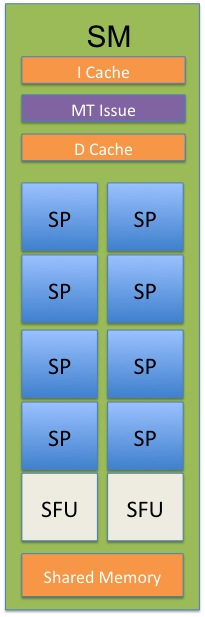
\includegraphics[height=80mm]{GPUdiagram1.jpg}
\caption{GT200 Architecture}
\label{GPUdiagram}
\end{figure}

The device's processors, shown in Figure \ref{GPUdiagram}, are
grouped hierarchically, with each level of the hierarchy sharing certain
hardware resources.  At the lowest level are symmetric processors or SPs, which
are very simple sequential shader processors.  At the next level are symmetric
multiprocessors or SMs, which are groups of 8 SPs that share an instruction
issue and decode unit.  This means that all SPs within an SM execute their
instructions in lockstep.  In the CUDA model, thread blocks are scheduled to run
in their entirety on a single SM.  The SPs are then grouped to share texture
processing units, and then these groups along with L2 caches make up the GPU
chip.  The graphics card bundles the GPU along with a large block of off-chip
DRAM, typically on the order of a few gigabytes in modern cards.

The CUDA model is a Single Instruction Multiple Thread or SIMT model, meaning
that multiple threads with a block each execute the same instruction at the same
time.  This differs from SIMD models in that branching instructions are allowed
which diverge with a thread block.  However, this results in a significant
performance degradation, as all threads in the block are then forced to execute
both paths of the branch, with logical noops being executed by the threads on
the path which didn't satisfy their conditional test.

In order to get maximum performance on a GPU, it is very important to manage
memory usage.  While the peak memory bandwidth on modern GPUs is up to 150GB/sec
or more--up to an order of magnitude higher than that of CPUs--this bandwidth
can only be reached with careful access patterns on the part of threads within a
block.  In addition, each SM has a 16KB scratchpad called {\it shared memory}.
The programmer must explicitly manage shared memory, and careful usage of it can
result in orders of magnitude performance improvements over naively-written CUDA
programs.  In addition, data must be manually moved between system RAM and the
graphics card's DRAM.  Modern GPUs use PCI-Express, which has a maximum transfer
rate of around 4GB/sec, which can easily become the major bottleneck in CUDA
programs if memory transfers aren't managed carefully.

Various constraints limit how a programmer can structure his or her CUDA
programs.  Each SM is able to execute a maximum of 8 thread blocks and a maximum
of 1024 threads at a time.  In addition, a group of thread blocks can be
co-scheduled on an SM only if they consume at most 16K registers, as each SM
shares a register pool.  Finally, no more than 16KB of shared memory per SM can
be used at a time, and so thread blocks with in aggregate exceed this limit
cannot be co-scheduled.

\section{Evaluation}
\label{Evaluation}

We evaluated Parakeet on two standard benchmark programs: Black-Scholes option
pricing, and K-Means Clustering.  We compare Parakeet against both hand-tuned
CPU and GPU implementations.  For Black-Scholes, the CPU implementation is
taken from the PARSEC \cite{Bien08} benchmark suite--which we used as the basis
of our Q implementation--and the GPU implementation is taken from the CUDA SDK
\cite{NvidSD}.  For K-Means Clustering, we wrote our own Q version in 17 lines
of code.  Both the CPU and GPU benchmark version come from the Rodinia
benchmark suite \cite{Che09}.

Our experimental setup is as follows.  We ran the CPU benchmarks on a machine
with 3 Intel Nehalem 2.67GHz X5650 4-core CPUs (for a total of 12 cores) with
24GB of RAM.  The peak throughput of this machine is thus 32GLOP/s, and it has
a peak memory bandwidth of 32GB/s.

For all GPU benchmarks, we ran the programs on both an NVIDIA GTX2XX and an
NVIDIA GTX460.  The GTX2XX has 240 processor cores with clock speeds of
Y.YY GHz and YMB of memory, with peak execution throughput of Y.YY GFLOP/s and
peak memory bandwidth of Y.YY GB/s.  The GTX460 has 336 processor cores with
clock speeds of 1.35GHz and 1GB of memory, and has a peak execution throughput
of 907 GFLOP/s and a peak memory bandwidth of 115.2 GB/s.

For our Parakeet benchmarks, the desktop system we used had a BLAH processor
with BLAH specs.

\subsection{Black-Scholes}


\subsection{K-Means Clustering}

\begin{figure}
\begin{verbatim}
calc_single_centroid: {[X;a;i] avg X[where a = i]}
calc_centroids:{[X;a;k]
  calc_single_centroid[X;a] each til k}
dist:{[x;y] sqrt sum (x-y) * (x-y)}
minidx:{[x] x ? min x}

kmeans:{[X;k;assignment;maxiters]
  C: calc_centroids[X;assignment;k];
  i: 0;
  converged: 0b;
  while[(i<maxiters) & not converged;
    lastAssignment: assignment;
    D: X dist/:\: C;
    assignment: minidx each D;
    C: calc_centroids[X;assignment;k];
    converged: all lastAssignment = assignment;
    i+: 1];
  (C; converged)}
\end{verbatim}
\caption{Q K-Means Clustering}
\label{QKMeans}
\end{figure}

\section{Related Work}
\label{RelatedWork}

There's Copperhead \cite{Cata10}.  They're almost as good as we are.

There has been much recent work dedicated to making parallel programming easier.
The various approaches to addressing this problem include libraries and APIs
which provide parallel functionality as well as new programming languages meant
for parallel programming.

Skeletons are cool \cite{Cole04}.

Recent work on parallel programming languages includes Fortress \cite{Alle08},
Unified Parallel C \cite{Char05}, and X10 \cite{Chen05}.  Our approach differs
from all of these in two important ways.  First, we are focusing on compiler
techniques for sequential array programming languages which do not require the
programmer to explicitly manage parallelism.  These techniques are meant to be
generally applicable to any suitable array language, not just Q.  Second, our
approach doesn't introduce a new programming language specifically for writing
GPGPU or parallel programs.  Q is already in wide use in the financial computing
community.

There has also been other work directed specifically at raising the level of
abstraction above that of CUDA and OpenCL for doing GPGPU programming.  Conal
Elliot's Vertigo \cite{Elli04} was a declarative parallel language embedded in
Haskell which was used for GPGPU programming.  It was designed for older GPUs
(pre-CUDA), and only parallelized map computations (not handling, for example,
parallel reductions or all-pairs type computations).  Microsoft's Accelerator
\cite{Tard06} is a declarative GPU language embedded in C\# which creates a
directed acyclic graph of LINQ operations--a collection of common data querying
operations such as filtering, grouping, and joining--and compiles them to
(pre-CUDA) shader programs.  Joel Svensson's Obsidian \cite{Sven08} is another
declarative language embedded in Haskell which compiles at runtime to the GPU.
The language semantics are inspired by hardware description languages and while
it is a higher level of abstraction than directly coding CUDA, it is still much
lower level than an array language such as Q.  Finally, Jacket by Accelereyes
\cite{AcceJa} provides a similar setup for Matlab as we do for Q.  However,
Jacket requires programmers to explicitly declare data and computation to reside
on the GPU, whereas our framework takes advantage of the GPU completely
transparently to the programmer.

Our approach is very similar in spirit to that of the skeletal programming
community \cite{Cole04}.  We both seek to use generic parallel programming
constructs which capture most of the common parallel patterns in a concise and
easy-to-use language.  In our specific case, these constructs are embodied by
Q's adverbs, which are second-order function modifiers.  We describe these
adverbs in more detail in the next section.

\section{Conclusion}
\label{Conclusion}

We have presented Parakeet, an intelligent runtime for executing high level
array-oriented programs on GPUs.  Parakeet alleviates programmers from having
to write code that explicitly manages low level architectural details, pushing
the level of abstraction for GPGPU programming up to the level of productivity
languages.  Parakeet automatically synthesizes GPU programs from data parallel
array operators, transparently running these programs and moving data back and
forth to the GPU's memory and performing GPU memory garbage collection.
Parakeet includes a series of optimizations to generate more efficient GPU
programs, including array operator fusion and the use of shared and texture
memory on the GPU.  Parakeet is a working system, in which complex programs can
be written and executed efficiently.  On two benchmark programs, Parakeet
delivers performance competitive with even hand-tuned CPU and GPU
implementations.

In future work, we hope to support more front ends and back ends.  At the
moment, we are building front ends for both Matlab and Python.  We envision
building a back end for multicore CPUs as well, likely targeting LLVM
\cite{Latt02}.

\bibliographystyle{acm}
\bibliography{../Parallelism}{}

\end{document}
